\documentclass{beamer}

\usepackage{listings}
\usepackage{color}
\definecolor{mygreen}{rgb}{0,0.6,0}
\definecolor{mygray}{rgb}{0.5,0.5,0.5}


% Beamer config
\setbeameroption{show notes} % {show notes} = print speaker notes
\usefonttheme{serif}
\usetheme{Berkeley}
\usecolortheme{seahorse}



% Set listings defaults
\lstset{    language=[LaTeX]TeX, 
            basicstyle=\scriptsize, 
            keywordstyle=\bfseries\color{blue}, 
            commentstyle=\it \color{red}, 
            stringstyle=\ttfamily, 
            numbers=left, 
            numberstyle=\tiny\color{mygray}, 
            numbersep=3pt, 
            literate= {\{}{{{\bf\color{mygreen}\{}}}1 {\}}{{{\bf\color{mygreen}\}}}}1 , 
            breaklines=true, 
            morekeywords={maketitle, subsubsection, subsection, thesection,}
        }

% define some commands

% \codeframe:  creates a frame with code on left and result (image) on right
% args: 1=Title on frame, 2=path to source, 3=path to image
\newcommand{\codeframe}[4]
{
    \begin{frame} \frametitle{#1}
        \begin{columns}[T]
            \column{.52\textwidth}
                \textbf{Source}
                \lstinputlisting[firstline=#3, lastline=#4]{Examples/#2.tex}
            \column{.46\textwidth}
                \textbf{Output}
                \fbox{\includegraphics[width=\textwidth]{Examples/#2.png}}
        \end{columns}
    \end{frame}
}

% \pc:  (stands for print command) having to type \textbackslash \{ \} every 
% time I want to include a LaTeX command is horrible.  This makes it less horrible.
\newcommand{\pc}[1]
{
    \texttt{\textbackslash #1}
}

% \pca:  (stands for print command (arg)) having to type \textbackslash \{ \} every 
% time I want to include a LaTeX command is horrible.  This makes it less horrible.
\newcommand{\pca}[2]
{
    \texttt{\textbackslash #1\{#2\}}
}

% Presentation Title block
\title{How do \LaTeX?}
\author{Eric Krause}
\institute[PSU]{Portland State University\\\it{M.S. ECE, 2013}}

\begin{document}
\maketitle

\section{Why \LaTeX?}


\begin{frame} \frametitle{Why use \LaTeX?}
    \begin{itemize}
        \item High quality output
        \item Unparalleled math/equation typesetting
        \item Powerful bibliography management 
        \item Handles massive documents with ease
        \item Free and OS agnostic
        \item You get to use your favorite text editor
        \item Highly extensible
        \item \textbf{Focus on content, not formatting}
    \end{itemize}
    
    \note{  -- Latex looks amazing.  MathType doesn't look as horrendous as it used to, but nothing beats latex for refinement/polish\\
            -- It is the mathematical typesetting standard in all technical disciplines and in many related fields. publications in math, computer  science, engineering, and physics\\
            -- this software is usually an extra expense (e.g. EndNote for Microsoft Word).  BibTex is fast, integrated, and powerful.\\
            -- once you start working on 20+ page documents with tons of pictures and tables (and partners, but that's another story) Word is simply not a viable option.  And by non-viable, I don't mean hard to use? I mean it will crash.  And if it doesn?t, you'll wish it did.\\
            -- Free, works on everything, in most if not all linux repos.\\
            -- plain text: vim, sublime text, notepad++, or even Emacs\\
            -- Tons of packages to do everything: code listing, create graphics, write music, whatever \\
            -- Most important:  Allows you to focus on content, not formatting.  \\
    }
\end{frame}


\begin{frame} \frametitle{Don't use LaTeX if...}
    \begin{itemize}
        \item Never used a computer before
        \item Can't spare a few hours of practice in exchange for a life changing skill
        \item Never need to create documents (why are you here?)
        \item Afraid of the command line
        \item Weak, lazy, other personal flaws
    \end{itemize}
    \note{in the beginning it might seem like it's too much work for short documents but with a little practice its really not bad and you'll find yourself using it even for simple things because \textbf{you know it will work every time}.  }
\end{frame}

\section{Getting Started}
\begin{frame} \frametitle{Downloading and Using \LaTeX}
    \textbf{Downloading}
    \begin{itemize}
        \item \textbf{Linux} Check your software repository.
        \begin{itemize} \item \texttt{sudo apt-get install texlive-full} \end{itemize}  
        \item \textbf{OS X} MacTex
        \begin{itemize} \item \url{http://www.tug.org/mactex/} \end{itemize}
        \item \textbf{Windows} ProTexT
        \begin{itemize} \item \url{http://www.tug.org/protext/} \end{itemize}
    \end{itemize}
        
    \textbf{Compiling [command line]}
    \begin{itemize}
        \item {\scriptsize \texttt{pdflatex -file-line-error -interaction=nonstopmode yourfile.tex}}
    \end{itemize}

    \textbf{Compiling [GUI]}
    \begin{itemize}
            \item Click buttons and/or mash keyboard.  
            \item If that doesn't work, try touching the screen or using voice commands.
    \end{itemize}
    \note{-file-line-error = file:line:error style messages. -interaction=nonstopmode = go back to command line on error. When pdflatex can't compile a file, it drops me to a prompt. I've never used it and always try to get away from there as quickly as possible, usually generating a q.log file in the process.
}
\end{frame}


\codeframe{Hello \LaTeX!}{1-hello}{1}{16}

\begin{frame} \frametitle{Syntax Example}
    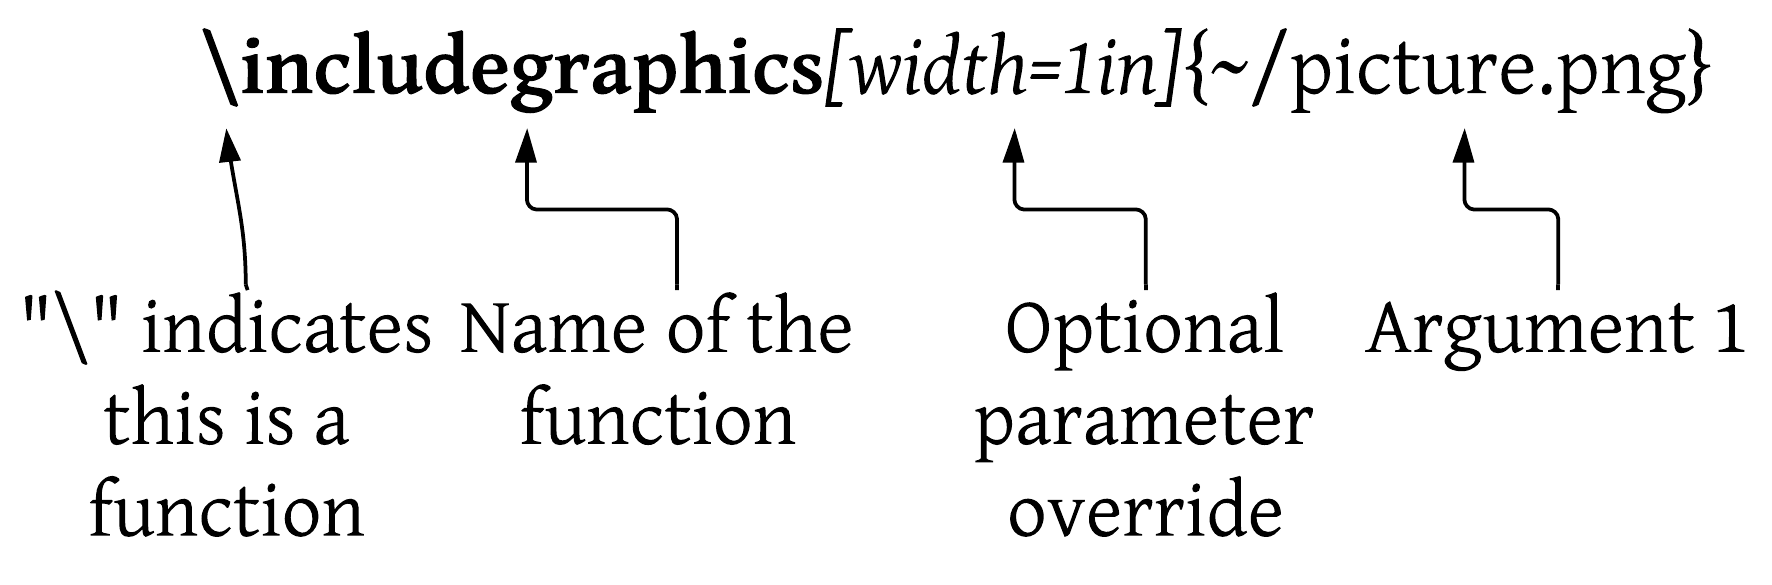
\includegraphics[width=\textwidth]{Examples/0-syntax.png}
\end{frame}

\begin{frame} \frametitle{Spaces and Escaped Characters}
\begin{itemize}
        \item Additional spaces between words are ignored.
        \item Manually add spaces by escaping a space \texttt{`\textbackslash\ '}
        \item Line break: (no indent) two backslashes \texttt{`\textbackslash\textbackslash'}
        \item Paragraph break (indent) two newlines (\texttt{`Enter'} twice)
    \end{itemize}
    
    \small
    \begin{tabular}{| l | l | l |} \hline
                            & \textbf{Unescaped Function}           & \textbf{To Print, Type:}  \\\hline
        \textbackslash      & escape character, command identifier  & \pc{textbackslash}        \\\hline
        \{ \}               & group and separate commands           & \pc{\{} and \pc{\}}       \\\hline
        \%                  & begin a line comment                  & \pc{\%}                   \\\hline
        \$                  & enter/leave math mode                 & \pc{\$}                   \\\hline
        \_                  & for subscripts (math mode)            & \pc{\_}                   \\\hline
        \textasciicircum    & for superscripts (math mode)          & \pc{textasciicircum}      \\\hline
        \&                  & designate columns in tables           & \pc{\&}                   \\\hline
        \#                  & reference arguments in functions      & \pc{\#}                   \\\hline
        \textasciitilde     & insert unbreakable space              & \pc{textasciitilde}       \\\hline
    \end{tabular}
    \note{point out that spaces are ignored and the difference between line breaking and paragraph breaking. not going to go through this in detail, basically backslash is escape character and also designates the start of a command or function.  }
\end{frame}


\section{Formatting}

\codeframe{Common Text Formatting}{2-formatting}{4}{10}

\codeframe{Sections and Subsections}{3-section}{5}{16}

\codeframe{Lists}{4-lists}{4}{19}

\begin{frame}
    \frametitle{Formatting Miscellanea}
    \begin{description}
        \item[Quotes] Backtick (\ \`\ ) for open quote, single quote (\ \'\ ) for close quote.  `single' or ``double''
        \item[Centering] \pca{begin}{center}\\ centered text\\ \pca{end}{center}
        \item[Verbatim] \pca{begin}{verbatim}\\ \ \ \ \ won't be parsed by \textbackslash LaTeX\\ \ \ \ \ great for console output\\\pca{end}{verbatim} 
    \end{description}
\end{frame}


\section{Math Mode}

\begin{frame} \frametitle{Math Mode}
    \begin{itemize}
        \item Begin/end inline equations with \$.
        \item Begin/end display equations with \pca{begin}{equation} and \pca{end}{equation}.
        \item Symbols accessed directly from the keyboard:  
        \begin{itemize} \item \textit{+ - = ! / ( ) [ ] $< >$ $|$ $'$ :} \end{itemize}
        \item \textbf{Dextrify to the rescue!}
        \begin{itemize} \item \url{http://detexify.kirelabs.org/classify.html} \end{itemize}
    \end{itemize}
    \note{There are lots of symbols in math, very few are accessed using keyboard in LaTeX.  The rest are all commands started with slash.  Hard to remember all of them, but with Dextrify they are easy to find if you can draw what you are looking for. }
\end{frame}

\begin{frame} \frametitle{Math Mode Examples}
    Output:
    \fbox{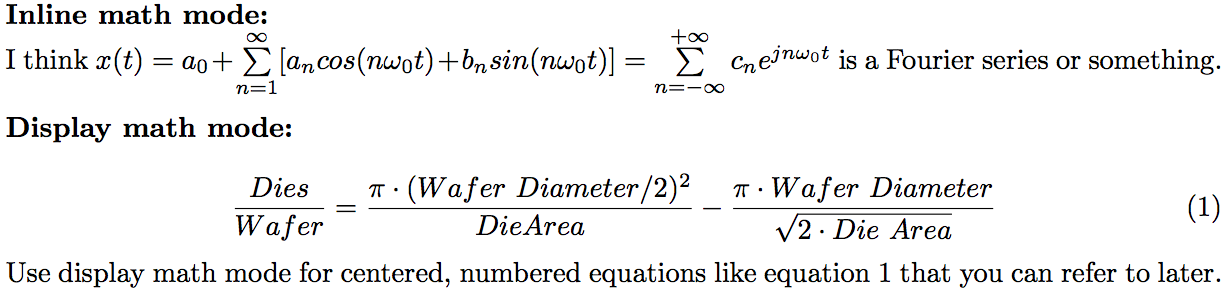
\includegraphics[width=\textwidth]{Examples/5-math.png}}

    Source:
    \lstinputlisting[basicstyle=\tiny, firstline=6, lastline=15]{Examples/5-math.tex}
    
    \note{probably too small to see, but this serves as a basic example.  Math is one of the strongest features in LaTeX, it can handle anything.}
\end{frame}


\section{Tabular Mode}

\begin{frame} \frametitle{Using the Tabular Environment}
    \begin{enumerate}
        \item \textbf{Begin tabular mode} specifying the number of columns, alignment, and vertical lines.
        \item \textbf{Input table rows} indicating separations between cells, specifying when to begin a new row, and where to include horizontal lines.
        \item \textbf{End tabular mode}
    \end{enumerate}
\end{frame}

\begin{frame} \frametitle{Beginning A Tabular Environment}
    Started using the following command:\\
    \ \ \ \ \ \pca{begin}{tabular}\texttt{\{column specification\}}\\
    \begin{itemize}
        \item The environment we are starting is \texttt{tabular}.
        \item The type, location, and alignment of columns and vertical lines is given using the \texttt{column specification}
	    \begin{itemize}
	        \item l --- left-aligned column
	        \item c --- center-aligned column
	        \item r --- right-aligned column
	        \item p\{width\} --- paragraph column, must specify width.
	        \item $|$ --- vertical line ($||$ = double, $|||$ = 	triple ...) 
	    \end{itemize}
    \end{itemize}
    \note{ Use paragraph columns to manually control column width.  Text will wrap in paragraph columns.\\\textit{(If text flows out of the table, try using this).}}
\end{frame}

\begin{frame} \frametitle{Adding Contents}
    \begin{itemize}
    	\item Once in a tabular environment, table contents, separations between cells, and newlines are entered.\\
    	\begin{itemize}
			\item \texttt{\&} --- column separator
			\item \texttt{\textbackslash\textbackslash} --- start new row
        	\item \pc{hline} --- horizontal line
			\item \pc{newline} --- start new line in cell (paragraph cells only)
		\end{itemize}
    \end{itemize}
    
    \textbf{Sample Table:}
    \lstinputlisting[firstline=5, lastline=11]{Examples/6-tables.tex}
\end{frame}

\begin{frame} \frametitle{Tabular Example}
    Output:
    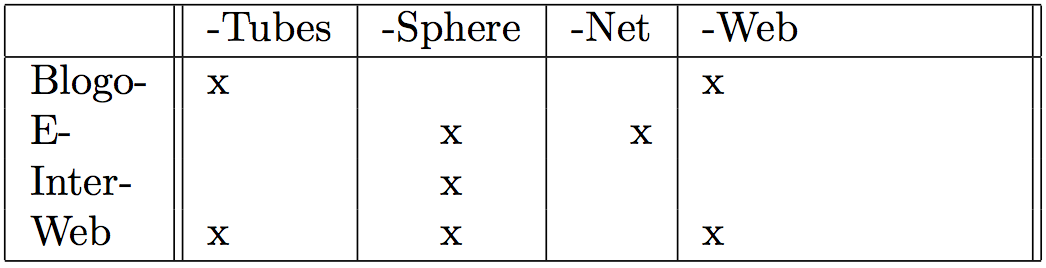
\includegraphics[width=\textwidth]{Examples/6-tables.png}
\end{frame}


\section{Graphics}
    \begin{frame}
    \frametitle{Importing Graphics}
    \begin{itemize}
        \item \texttt{\textbackslash usepackage graphicx}
        \item Once \texttt{graphics} is included, images are imported using:\\\vspace{6pt}\pc{includegraphics}\textit{[optional params]}\{image name\}\vspace{6pt}
        \item Useful optional parameters:
        \begin{itemize}
            \item width=xx --- manual width
            \item height=xx --- manual height
            \item angle=xx --- used to rotate image
            \item scale=xx --- manual scaling
        \end{itemize}
            
        \item width=\pc{textwidth}: full-page-width picture
        \item width=0.5\pc{textwidth}: half-page-width picture
    \end{itemize}
    \note{LaTeX cannot manage pictures directly, must use the \texttt{graphicx} package. Add to preamble of document:\\ }
\end{frame}

\codeframe{Includegraphics Example}{7-images}{1}{6}


\section{Floats}

\begin{frame} \frametitle{Floats}
    \begin{itemize}
        \item A float is a container that cannot be broken across multiple pages
        \item \LaTeX\ defines \texttt{figure} and \texttt{table} floats
        \item Floats have captions and references.
        \item Floats are automatically arranged by \LaTeX\ (however, you can manually specify placement)
    \end{itemize}
\end{frame}

\begin{frame} \frametitle{Float Placement}
    \textbf{Format:}\\
    \pca{begin}{figure}\textit{[placement specifier]}\\
    \ \ \pc{label} \{fig:cat\}\\
    \ \ \pc{caption} \{ this is a photo of a cat \}\\
    \ \ ... figure contents ...\\
    \pca{end}{figure}

    \begin{itemize}
        \item Placement Specifiers 
        \begin{itemize}
            \item h --- Place the float (approximately) here
            \item t --- Position at the top of the page.
            \item b --- Position at the bottom of the page.
            \item p --- Put on a special page for floats only.
            \item ! --- Override internal parameters LaTeX uses for determining "good" float positions.
        \end{itemize}
    \end{itemize}
    \note{Label and caption can go before or after figure contents. 
}
\end{frame}

\codeframe{Floats Example}{8-floats}{6}{23}


\section{Code Listings}
    \begin{frame}
    \frametitle{Listings}
    \begin{itemize}
    	\item \pca{usepackage}{listings}
        \item Made specifically for listing source code. 
        \item Syntax highlighting for all common languages.
        \item (Bad) Write/paste code into \LaTeX\ document: \\
        \ \ \ \ \pca{begin}{lstlisting}\\ \ \ \ \ \ \ \ \ Put your code here\\ \ \ \ \ \pca{end}{lstlisting}
        \item (Good) Reference original source file: \\
        \ \ \ \ \pc{lstinputlisting}\texttt{[options]\{path\_to\_file\}}
        \item \url{http://en.wikibooks.org/wiki/LaTeX/Source\_Code\_Listings\#Settings}
    \end{itemize}
    \note{The verbatim environment is useful for non-formatted text like console output but with listings you will get beautiful syntax highlighting that looks good printed in color or b/w, or on screen}
\end{frame}

\codeframe{Listing Example}{9-listing}{R}{}

\section{BibTex}

\section{Useful Packages}

\end{document}
       